\documentclass{article}
\usepackage{v-problem}
\vgeometry

\begin{document}
\vtitle[ELECTROSTATICS]

\def\pn{03}
\def\book{Irodov}
\def\page{105}
\def\gdrive{https://drive.google.com/drive/folders/1gUoLRu1eSusnIVRXYnN6m10F0xXTeOkR?usp=share_link}

\def\question{
What would be the interaction force between two copper spheres, each of mass $1 \gm$, separated by the distance $1 \m$, if the total electronic charge in them differed from the total charge of the nuclei by one per cent?
}

\vspace*{\fill}
\begin{tikzpicture}
	\node[qnumber] (n) at (0, 0)[scale=2] {$\pn.$};
	\node[question] (q) [right=2mm of n.east] {\question};
	\tzline[divider]<-0.125, 0> (q.north west)(q.south west);
	\node[format] (f) at  (q.south east){[\book \quad \page]};
\end{tikzpicture}	
\vspace*{\fill}

\begin{center}
\begin{tikzpicture}
\tzcoor*[black!50](0, 0)(Q1){$1\gm$}[bl](15pt)
\tzcoor*[black!50](5, 0)(Q2){$1\gm$}[br](15pt)
	\tzline[|<->|]<0, -0.5>(Q1)(Q2){$1\m$}[mb]
	\tzdots*(Q1)(Q2);(5pt)
\end{tikzpicture}
\end{center}
\vspace*{\fill}
\pagebreak

\vtitle[\texttt{Solution}]
\addtolength{\jot}{2ex}
\begin{align*}
\intertext{Total nuclear charge in $1\gm$ of copper}
Q &= \dfrac{1}{A} \cdot N \cdot e \cdot Z\\
\intertext{$A_{C\!u}=63.54, \quad N=\kAvogadro, \quad e=\kChargeFundamental, \quad Z_{C\!u}=29$}
	&= \dfrac{1}{63.54} \times 6.02 \times 10^{23} \times 1.6 \times 10^{-19} \times 29\\
	&= 4.398 \times 10^4 C
\end{align*}

\begin{align*}
\intertext{Charge on single sphere}
q &= 1\% \textit{ of } Q\\
	&= \dfrac{1}{100} \times 4.398 \times 10^{4} C\\
	&= 4.398\times10^2 C
\end{align*}

\begin{align*}
\intertext{Electrostatic force between these two spheres}
F_e &= \dfrac{1}{4\pi\varepsilon_0} \cdot \dfrac{q^2}{r^2} \\
	&= 9\times10^9 \cdot \dfrac{\left(4.398\times10^2\right)^2}{1^2}\\
	&= 1.74 \times 10^{15} \N \ans
\end{align*}

\pagebreak

\vspace*{\fill}
\begin{center}
	\fbox{\qrcode[height=2cm]{\gdrive}}
\end{center}
\vspace*{\fill}

\end{document}
